\documentclass{article}
%%%%%%%%%%%%%%%%%%%%%%%%%%%%%%%%%%%%%%%%%%%%%%%%%%%%%%%%%%%%
\usepackage{graphicx} % Required for inserting images
\usepackage{neurips_2023}
%%%%%%%%%%%%%%%%%%%%%%%%%%%%%%%%%%%%%%%%%%%%%%%%%%%%%%%%%%%%
\usepackage[utf8]{inputenc} % allow utf-8 input
\usepackage[T1]{fontenc}    % use 8-bit T1 fonts
\usepackage{hyperref}       % hyperlinks
\usepackage{url}            % simple URL typesetting
\usepackage{booktabs}       % professional-quality tables
\usepackage{amsfonts}       % blackboard math symbols
\usepackage{nicefrac}       % compact symbols for 1/2, etc.
\usepackage{microtype}      % microtypography
\usepackage{xcolor}         % colors
\usepackage{kotex}
\usepackage{float}

%%%%%%%%%%%%%%%%%%%%%%%%%%%%%%%%%%%%%%%%%%%%%%%%%%%%%%%%%%%%

\title{RoBaMF : Role-Based Multimodal Fusion model\\
for Online News Classification}
\author{M.S Park, J.H ahn, L.S Yoon}
\date{October 2023}

\begin{document}

\maketitle

\begin{abstract}
  The transmission of information is not limited to text, but also includes various forms such as images, videos and voices. Thus, the use of multimodal models in data analysis is gaining attention. In this paper, we propose a multimodal model called RoBaMF that reflects both text data and image data from online newspapers in the analysis. The RoBaMF includes a feature-fusion model to reflect the interaction between images and annotations. Additionally, we consider an ensemble methodology that also takes into account single models of text and images. According to our research results, RoBaMF did not improve accuracy compared to article-image composite models, due to some limitations.
\end{abstract}

\section{Introduction}
Internet news articles consist of a title, main text, images, and annotations for those images. To categorize these articles, it is reasonable to consider a multimodal model that incorporates both text and image information into the analysis. Moreover, since annotations provide detailed descriptions of the images, there is a strong correlation between images and their accompanying annotations. In this paper, we propose the RoBaMF model, which includes the role of annotations in solving the news article category classification problem. This model incorporates base classifiers using feature-fusion to reflect the interaction between images and their associated annotations. In addition, to reflect the unique information from the article text and images - both of which play significant roles in newspapers - we have incorporated individual base classifiers for each element. The results were produced by applying ensemble methods to these three base classifiers.



\section{Related Work}
\subsection{News classification based on text information}
Suh Y, Yu J, Mo J, Song L. (2017) conducted category classification based on Naver article data using Logistic Regression (LR), SVM, Naïve Bayes, and KNN. Yoon (2014) proposed TextCNN, a CNN document classification model that uses word embedding matrices as input values\cite{suh2017comparison}. Jang B, Kim I, Kim JW (2019) performed tweet and news classification using Word2Vec and CNNs and demonstrated that Word2Vec improves performance by learning semantic relationships between words\cite{jang2019word2vec}. Nishant Rai, Deepika Kumar, Naman Kaushik, Chandan Raj, Ahad Ali (2022) combined BERT with LSTM to perform fake news classification\cite{rai2022fake}.


\subsection{Feature Fusion}
Feature fusion refers to the process of merging information extracted from (integrating disparate data sources into a unified representation)or(two different data sources into one), transforming heterogeneous features into a single vector. Simple methods of feature fusion include maximization, summation, and concatenation. Nicolas Audebert, Catherine Herold, Kuider Slimani, Cédric Vidal (2019) employed the concatenation method in their image-text multimodal classification problem\cite{audebert2020multimodal}. In their paper, they stated that models using the summation method performed worse than those using only images (pure-image model), inferring that this was due to summation undermining the unique discriminating power of both images and text. As for more complex feature-fusion methods, Jian Yang (2002) proposed parallel feature fusion\cite{yang2003feature} while Yimian Dai (2021) suggested attentional feature fusion\cite{dai2021attentional}.


\subsection{Ensemble methods}
Ensemble methodology is a technique that combines multiple base models to improve the accuracy of predictions. Yawen Xiao, Jun Wu, Zongli Lin, and Xiadong Zhao (2017) presented a deep learning-based multi-model ensemble methodology that demonstrated excellent results\cite{xiao2018deep}. In a study by Silvia Corchs, Elisabetta Fersini \& Francesca (2019), they conducted sentiment analysis applying the BMA (Bayesian Model Averaging) ensemble methodology to image-text multimodal data\cite{corchs2019ensemble}.


\section{Methodology}
\subsection{Textual Features}
In this study, we need to extract features from text data, which includes the title and body text. To do this, we use KoBERT for extracting textual features.
KoBERT, like the original BERT\cite{devlin2018bert}, adopts a Masked Language Model that masks some words and predicts those masked words during training to extract context information in both directions of the input sequence.
KoBERT was developed to overcome some limitations in Korean NLP performance of the existing BERT-base multilingual cased (hereafter MBERT). It was trained on a corpus composed of Korean sentences collected from sources such as Wikipedia and news articles.
To reflect unique changes in the Korean language, it applies the SentencePiece tokenizer that can handle a long sentence as a single token.
KoBERT has shown about 27\% performance improvement in Korean NLP compared to MBERT.
In practice, KoBERT showed superior results than MBERT in sentiment analysis for reviews on a Korean e-commerce platform and for corporate-related Korean news.




\subsection{Visual features}
Using visual features extracted by fine-tuned deep CNNs can be an excellent baseline for visual recognition tasks\cite{sharif2014cnn}. Based on this, we extract deep visual features from news images using fine-tuned MobileNetV2 with ImageNet in this study. MobileNetV2 is a successor model to MobileNet that improves performance while reducing model size and computational load by adopting an inverted residual structure. It consists of stacked bottleneck blocks that sequentially perform the following three stages: narrow pointwise convolution followed by identity activation; 3 by 3 wide depthwise separable convolution followed by ReLU activation; narrow pointwise convolution followed by ReLU activation again. Ke Dong, Chenjie Zhou, Yihan Ruan \& Yuzhi Li (2020) showed better results performing image classification using MobileNet V2 compared to previous models\cite{dong2020mobilenetv2}.



\subsection{Feature fusion}
In this research, image features were first extracted using MobileNetV2, and text features were obtained using KoBERT. These features were then input into a feedforward NN model. "To do so, two feature vectors were combined by stacking them together into a single vector."
This feature fusion method, known as concatenation, has several advantages:\\

\textbf{1. Information Preservation}\\
Concatenation simply connects feature vectors without the need to consider the size or characteristics of the two feature vectors being combined. As a result, it completely retains the features derived from each domain, minimizing information loss. Therefore, it is advantageous for multi-modal data that requires the preservation of the discriminating power of each domain.\\

\textbf{2. Flexibility}\\
Concatenation remains unaffected even if the feature extraction method (feature extractor) is changed. For example, in this paper, it is possible to replace MobileNetV2, which is considered for image feature extraction, with another state-of-the-art deep CNN model like ResNet.\\


\subsection{Ensemble Methods}
This research aims not only to consider interactions between images and annotations but also to consider unique information contained within articles and images.
Additionally, we intend to understand the impact of the interaction between images and annotations on the performance of the model in news category classification problem.
To address both these considerations, weighted soft-voting ensemble and stacking ensemble methodology were applied onto the final model.
Unlike traditional soft-voting that simply sums up prediction probabilities of base classifiers, weighted soft-voting assigns weights based on classification performance of the base models.
Therefore, it allows us to assess the impact of the interaction between images and annotations on the classification performance through these weights.
The stacking ensemble methodology uses the prediction probabilities from base classifiers (level 1 classifiers) as input for a meta model (level 2 classifier or meta learner). Using XGBoost, which is based on decision trees, as a meta-model, we can calculate the importance of features. This  allows us to understand the effect of image-annotation interaction models on classification.
The multimodal classification model created by these processes is referred to as the Role-Based Multimodal Fusion Model (RoBaMF). The overall pipeline of the RoBaMF model is shown in Figure 1.

\begin{figure}[ht]
    \centering
    \includegraphics[width=\columnwidth]{ENG/fig.1.jpg}
    \caption{The overall pipeline of the RoBaMF model}
    \label{fig.1}
\end{figure}


\section{Experiments}
\subsection{Dataset}
The Naver internet news aggregator is divided into six main categories: Politics, Economy, Society, Life/Culture, IT/Science and World. News without images were excluded from the crawling target. Also, news containing data that did not fit this research was filtered out after crawling.
We extracted the category, title, body, and image-annotation pairs from a single article
A total of 12920 news items were included in the dataset. We randomly selected 1200 news from each category to be used as training data, and the remaining were used as test data.



\subsection{Models}
This subsection describes the implementation of our RoBaMF model along with some comparative models. All models are implemented in PyTorch.




\textbf{Article Text Baseline}\quad
The KoBERT model is used to extract information from title and body text.
The input dataset consists of a list of ['title + body', 'category'] for each article.
Since we perform classification for six categories in this study, a vector of length 6 is appended to the output layer.
From now on, this model will be referred to as "Article".



\textbf{Image Baseline}\quad
The MobileNetV2 model is used to extract information from photos and diagrams.
Pre-trained weights on ImageNet are loaded which enhances the discriminating power of image features through such transfer learning.
The MobileNetV2 feature extractor was followed by classification dense layers with lengths of 1024, 1024, and 6 respectively.
Also, image sizes are adjusted to (224, 224, 3) to match the input format of MobileNetV2. 
From now on this model will be referred to as "Image".

%
\begin{figure}[ht]
    \centering
    \begin{minipage}{0.48\textwidth}
        \centering
        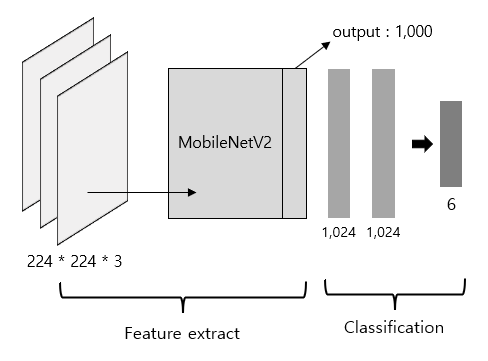
\includegraphics[width=6cm]{ENG/image-baseline.png} % Second figure file
        \caption{Image baseline}
        \label{fig.2}
        
    \end{minipage}\hfill
    \begin{minipage}{0.48\textwidth}
        \centering
        \includegraphics[width=6cm]{ENG/text-baseline.png} % First figure file
        \caption{Article text baseline}
        \label{fig.3}
    \end{minipage}
\end{figure}
%

\textbf{Feature Fusion Baseline}\quad
This is a model designed to ascertain the discriminative power of image-text multimodal features. 
Text and images are separately input into KoBERT and MobileNetV2, and features from both domains are extracted by setting the output layer length to 1024. 
The concatenate method was applied to fusion the features from both domains into a vector of length 2048, followed by classification dense layers of lengths 2048, 1024 and 6, respectively.
The model using article text data will be referred as "Article-Fusion" and one using annotation text will be called "Annotation-Fusion".

\begin{figure}[ht]
    \centering
    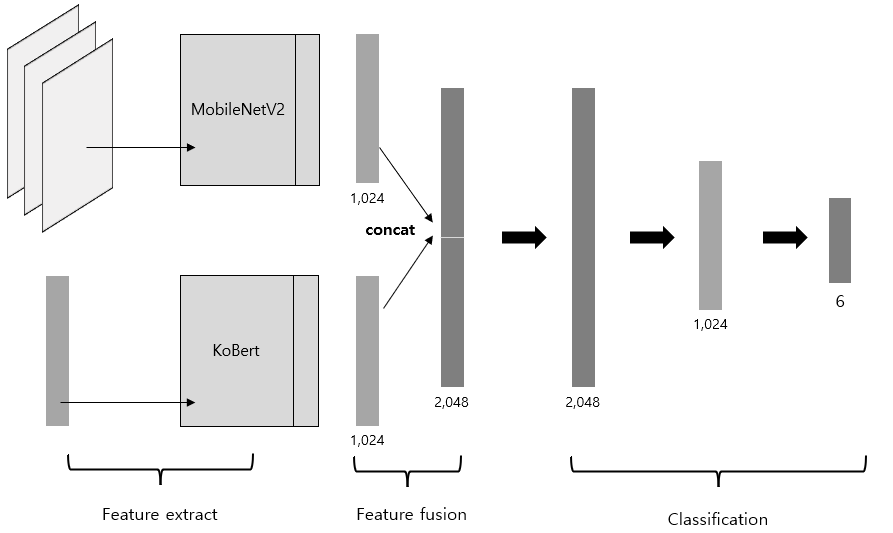
\includegraphics[width=8cm]{ENG/feature-fusion-baseline.png}
    \caption{Feature Fusion baseline}
    \label{fig.4}
\end{figure}

\textbf{Ensemble Competitor Models}\quad
This is a competing model designed to compare the performance of the proposed RoBaMF model in this study. It utilizes the Article, Image, Article -Fusion model as the base classifiers and implements the K-fold stacking ensemble methodology. It uses XGBoost as a meta-learner. This model is called Competitor.


\textbf{RoBaMF Model}\quad
This is the model that considers two unique features of articles and images, as well as the interactions between images and annotations. It utilizes the Article, Image, Annotation-Fusion model as the base classifiers and implements the K-fold stacking ensemble methodology. Same as Competitor, it uses XGBoost as a meta-learner. This model is called RoBaMF.


\textbf{K-fold Cross Validation}\quad
To determine the optimal hyperparameters for each baseline, we employed K-fold cross-validation. For each fold, the training data was divided again into 5,760 training data and 1,440 validation data to train the baselines. Trained weights of the baselines were saved for the K-fold stacking ensemble, which we will discuss later. The performances of baseline models were pre-evaluated by averaging the accuracies across five folds (5-fold CV Accuracy). Subsequently, after tuning the optimal hyperparameters and training the model with the training data, predictions were made on the test data to calculate the accuracy (Test data prediction Accuracy).

\textbf{K-fold Stacking Ensemble}\quad
Both Competitor and RoBaMF model, a cross-validated stacking ensemble approach was implemented. Trained weights from K-fold CV were utilized to compute predictions for both the validation and test datasets across each fold. The predictions of the validation data were concatenated row-wise to serve as the meta-feature training data for the meta-learner, while the predictions of the test data were aggregated to form the meta-feature test data for the meta-learner. We used the accuracy on the meta-feature test data as the test data prediction accuracy of ensemble models.

\section{Result}
The K-fold CV accuracies of all baseline classifiers can be seen in Fig.5, and the test data prediction accuracies of all models are presented in Fig.6.

\begin{figure}[ht]
    \centering
    \begin{minipage}{0.48\textwidth}
        \centering
        \includegraphics[width=7.5cm]{ENG/fig. 2.png} % First figure file
        \caption{K-fold CV accuracy of all baseline classifiers}
        \label{fig.5}
    \end{minipage}\hfill
    \begin{minipage}{0.48\textwidth}
        \centering
        \includegraphics[width=7.5cm]{ENG/test-data-preds.png} % Second figure file
        \caption{Test data predictions accuracy.}
        \label{fig.6}
    \end{minipage}
\end{figure}



\subsection{Cross-Validation Accuracy for Baseline Models}
\textbf{<Low Decision Power of Image Baseline Classifier>} \\
The image baseline classifier, which utilized MobileNetV2 for feature extraction, demonstrated a cross-validation accuracy and test data prediction accuracy below 40\%. The poor discriminating power of the image baseline classifier is presumed to stem from the ambiguity of image data. For example, a photo of the president Yoon, as shown in Fig.7, might be expected to fall under the 'politics' category but is actually included in the 'life' category. Furthermore, government symbols, brand logos, and portraits, similar to those in Fig.8, are distributed across all categories, complicating accurate classification.

\begin{figure}[ht]
    \centering
    \begin{minipage}{0.48\textwidth}
        \centering
        \includegraphics[width=6cm]{ENG/fig.4-1.png} % Second figure file
        \caption{A picture containing ambiguous imformation}
        \label{fig.7}
        
    \end{minipage}\hfill
    \begin{minipage}{0.48\textwidth}
        \centering
        \includegraphics[width=6cm]{ENG/fig.4-2.jpg} % First figure file
        \caption{A picture containing ambiguous imformation 2}
        \label{fig.8}
    \end{minipage}
\end{figure}



\textbf{<Limitations of the Fusion Baseline Classifier>} \\
The Article-Fusion baseline classifier exhibited a slightly lower accuracy than the Article baseline. Despite the application of concatenation, it is conjectured that the combination of features from the two modalities might have led to a degradation of their unique discriminating power, resulting in such a phenomenon. Alternatively, it might be due to the selection of optimizers or hyperparameters for the multimodality. \\
The Annotation-Fusion Baseline classifier performed significantly worse than the Article-Fusion baseline classifier. Most of the annotations are less than 15 words long, it is likely that the KoBERT feature extractor was unable to extract meaningful features due to the limited information they contain compared to articles.

\subsection{RoBaMF and Competitor}
The importance of each baseline in two ensemble models can be found in Table 1, Table 2 and Fig.9.
The RoBaMF model performed equally or slightly better than the Article baseline, The Competitor model improved the test data prediction accuracy about 1\%p
The poor performance of the RoBaMF model, despite using more data, is due to the difference in discriminating power between the Annotation-Fusion and Article-Fusion baseline classifier.
This is supported by the baseline importance of both models.
For the RoBaMF model, the Annotation-Fusion baseline has an average importance of 11\%, while for the Competitor model, the Article-Fusion baseline has an average importance of 28\%.
Furthermore, both models show that the importance of the Article baseline classifier is much higher than the other baselines, confirming that the Image baseline and Fusion baseline are not decisive enough.

\begin{table}[htbp]
\centering
\begin{minipage}[t]{0.45\textwidth}
\centering
\caption{Competitor}
\label{tab:competitor}
\begin{tabular}{@{}lllllll@{}}
\toprule
Condition       & \multicolumn{1}{c|}{ACC} & \multicolumn{3}{c}{Importance} \\
             & Value      & Image      & Article      & Fusion     \\
\midrule
Condition 1   & 0.745         & 0.003         & 0.699         & 0.297       \\
Condition 2   & 0.745         & 0.011         & 0.565         & 0.423       \\
Condition 3   & 0.750         & 0.001         & 0.751         & 0.247       \\
Condition 4   & 0.748         & 0.0008        & 0.819         & 0.179       \\
Condition 5   & 0.747         & 0.0002        & 0.751         & 0.248       \\
\bottomrule
\end{tabular}
\end{minipage}
\hfill
\begin{minipage}[t]{0.45\textwidth}
\centering
\caption{RoBaMF}
\label{tab:robamf}
\begin{tabular}{@{}lllllll@{}}
\toprule
Condition       & \multicolumn{1}{c|}{ACC} & \multicolumn{3}{c}{Importance} \\
             & Value      & Image      & Article      & Fusion     \\
\midrule
Condition 1   & 0.740         & 0.001         & 0.884         & 0.113       \\
Condition 2   & 0.738         & 0.010         & 0.780         & 0.209       \\
Condition 3   & 0.739         & 0              & 0.913         & 0.087       \\
Condition 4   & 0.739         & 0.0005        & 0.976         & 0.023       \\
Condition 5   & 0.739         & 0.0002        & 0.876         & 0.123       \\
\bottomrule
\end{tabular}
\end{minipage}
\end{table}


\begin{figure}[ht]
    \centering
    \includegraphics[width=8cm]{ENG/importance.png}
    \caption{Importance}
    \label{fig.last}
\end{figure}


\begin{table}[htbp]
\centering
\caption{XGBoost : Hyper parameters}
\label{your-label}
\begin{tabular}{@{}lllllll@{}}
\toprule
Conditon     & \multicolumn{2}{c}{Hyper parameter} \\
             & n      & lr      & lambda      & max-depth     \\
Condition 1   & 50         & 0.05         & 100         & 4        \\
Condition 2   & 500         & 0.05         & 500         & 5       \\
Condition 3   & 100         & 0.01         & 100         & 3       \\
Condition 4   & 100         & 0.001        & 100         & 4       \\
Condition 5   & 200         & 0.01        & 1000         & 5       \\
\bottomrule
\end{tabular}
\end{table}

\section{Conclusion}
Image baseline has a low performance due to ambiguous image data. Fusion baseline has lower accuracy rates than Article baseline due to the loss of discriminating power caused by feature concatenation or failure of choosing optimizer and optimal hyperparameters. Also, annotation fusion baseline performed worse due to the lack of information in annotation texts.
The RoBaMF model used more data than the Competitor model, but performed worse due to the difference in discriminating power of the two fusion baselines.
Future research might consider how features can be fused in news data without compromising the own discriminating power of the two modalities.
It should also be investigated whether news-specific pre-training, such as KLUE-BERT, can overcome the limited information in annotation texts.



\bibliography{ref}
\bibliographystyle{plain}



\end{document}
